\section[Jednotky a veličiny v dozimetrii]{Jednotky a veličiny v dozimetrii, základy legální metrologie, etalony a stanovená měřidla}

Metrologie je věda zabývající se měřením . Mezi základní cíle a úkoly patří:

\begin{itemize}
    \item definice jednotek a jejich realizace pomocí vědeckých metod,
    \item vývoj a udržování etalonů nejvyšší úrovně,
    \item zajištění fungování měřidel ve výrobní sféře,
    \item zajistit správnost měření v úředních nebo obchodních sférách,
\end{itemize}

\subsection{Základy legální metrologie}

Hlavním je zákon č. 505/1990 Sb. o metrologii $\rightarrow$ upravuje práva a povinnosti subjektů a státních orgánů správy pro účely zajištění správnosti a jednotnosti měřidel a měření.
Dále jsou důležité prováděcí vyhlášky k samotnému zákonu, a to sice:

\begin{itemize}
    \item Vyhláška MPO č. 262/2000 Sb., kterou je zajišťována jednotnost a správnost měřidel a měření.
    \item Vyhláška MPO č. 345/2002 Sb., kterou se stanoví měřidla k povinnému ověřování a měřidla podléhající schvalování.
    \item Vyhláška MPO č. 264/2000 Sb., o základních měřících jednotkách a ostatních jednotkách a o jejich označování.
\end{itemize}

Klasifikace měřidel:

\begin{itemize}
    \item \textbf{Etalony} (primární, sekundární, mezinárodní, státní) = objekt či něco jiného, jež obecně slouží k uchování a realizaci dané jednotky (etalon hmotnosti, kde jednotka je kg, tak je snad krystal křemíku, protože umíme přesně určit počet atomů v mřížce).
    \item \textbf{Stanovená měřidla} = Jedná se o měřidla, která MPO (ministerstvo průmyslu a obchodu) vyhláškou stanoví k povinnému ověřování s ohledem na jejich význam (obchod, daně, sankce, tarify, poplatky, medicína, ochrana ŽP, BOZP).
    \item \textbf{Pracovní měřidla} = jedná se o měřidla jež nejsou etalonem ani stanoveným měřidlem.
    \item \textbf{Certifikované a ostatní referenční materiály} = Jedná se o materiály přesně stanoveného a známého chemického složení, které slouží pro ověřování nebo ke kalibraci (často to bývají etalony)
\end{itemize}

Schvalování typů měřidel je proces, při kterém jsou ověřeny metrologické a technické vlastnosti stanovených měřidel, jež vycházejí z technických norem. Zkoušky pro schválení typu stanoveného měřidla obsahuji funkční zkoušky, zkoušky odolnosti proti rušivým vlivům vnějšího prostředí a zkoušky elektromagnetické kompatibility. Výsledkem je certifikát a přidělení značky schválení typu.

Pod pojmem \textbf{návaznost} rozumíme: (definice je na hovno) V zásadě se jedná o to, že vemu např. 8 vah z celého světa, nastavím je pomocí kvalitního etalonu na to, že toto je 1 kg a potom, když něco naměřím já, tak i Karlíkovi z horní dolní můžu věřit, že to má jak já, protože to má nastavený v návaznosti na ten samý etalon a tudíž i v návaznosti na mne.

\textbf{Ověřování} je proces, resp. potvrzení, že měřidlo má požadované metrologické vlastnosti.

\textbf{Kalibrace} je proces, kdy je periodicky upravováno a kontrolováno, že měřidlo měří to co má a případná kalibrace probíhá pomocí certifikovaných a ostatních referenčních materiálu, kterými jsou nejčastěji etalony.

\subsubsection{Organizace}

\textbf{ÚNMZ = Ústav pro technickou normalizaci, metrologii a státní zkušebnictví}

\begin{itemize}
    \item Zastupování ČR ve věci mezinárodních věcí s ohledem na metrologii.
    \item Dohled na činnosti ČMI.
    \item Kontrola dodržování zákona o metrologii.
    \item Schválení a vyhlášení státních etalonů.
    \item Poskytování metrologických expertíz.
\end{itemize}

\textbf{ČMI}

\begin{itemize}
    \item Uchovávání a rozvoj státních etalonů.
    \item Schvalování typů a ověřování stanovených měřidel.
    \item Certifikace referenčních materiálů.
    \item Kalibrační služby.
\end{itemize}

\subsubsection{Veličiny a jednotky}

Existují různé soustavy jednotek, kde nejvíce je rozšířené SI, dále existuje imperiální, americká apod... Stačí znát SI.

V obecnosti jsou základní jednotky SI popsáné v Zákoně č. 505/1999 Sb. o metrologii. Obsaženy jsou dále odvozené jednotky, násobky, díky a jiné povolené jednotky.

Základní jednotky a veličiny SI jsou:

\begin{itemize}
    \item Čas -- s,
    \item Proud -- A,
    \item Svítivost -- cd,
    \item Látkové množství -- mol,
    \item Teplota -- K,
    \item Hmotnost -- kg,
    \item Délka -- m.
\end{itemize}

Odvozené jednotky vyjadřované jednotkami základními jsou např. hustota, objem, plocha, rychlost, ...

Odvozené jednotky se zvláštním označením i názvem jsou např. náboj, síla, aktivita, absorbovaná dávka, ...

Odvozené jednotky vyjádřené jednotkami základními spolu s jednotkami se zvláštním názvem a označením jsou např. Expozice, PDE, dávkový příkon, dávkový ekvivalent, ...

\textbf{Vlastnosti a výhody SI:}

\begin{itemize}
    \item Systematická a mezinárodně uznávaná soustava veličin a jednotek.
    \item Pro každou veličinu zavedena pouze jedna jednotka.
    \item Odvozené jednotky tvořeny součiny mocnin základních jednotek.
    \item Násobky a díly jednotek vyjádřeny předponami.
\end{itemize}

\textbf{Další mimosoustavné jednotky:} Jsou použitelné spolu s SI v rámci specifikovaných oborů a nebo výjimečně a tehdy, jeli definován vztah k SI jednotkám: uzel, dioptrie, angstrom, barn, atm, curie, calorie.

\textbf{Veličiny ve vztahu k atomové a jaderné fyzice:} Aktivita, přeměnová konstanta, poločas rozpadu, barn, hustota toku, fluence, absorbovaná dávka, kerma, expozice, dávkový ekvivalent, efektivní dávka, PDE, ...

\subsection{Jednotky a veličiny v dozimetrii}

\textbf{Expozice:}

Definována pro popis ionizujících účinků fotonů ve vzduchu: $[X] = C \cdot \text{kg}^{-1}$.

Expozice je definována jako podíl celkového náboje d$Q$ iontů jednoho znaménka, jež vznikly při úplném zabrzdění všech elektronů a pozitronů uvolněných fotony v malém objemu vzduchu, a hmotnosti tohoto objemu vzduchu d$m$.

\begin{equation}
    X = \frac{\text{d}Q}{\text{d}m}
\end{equation}

\begin{figure}[H]
    \centering
    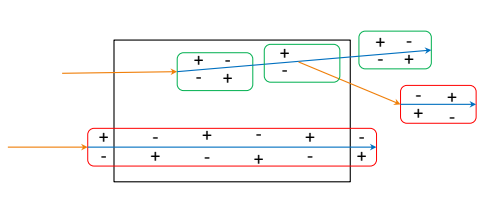
\includegraphics[width=0.5\linewidth]{img/expozice.png}
    \caption{expozice}
\end{figure}

\textbf{Absorbovaná dávka}

Vyjadřuje střední energii předanou IZ dané látce o jednotkové hmotnosti: $[D] = \text{Gy}$.

\begin{equation}
    D = \frac{\text{d}\overline{\varepsilon}}{\text{d}m}
\end{equation}

\textbf{Kerma}

Popisuje působení nepřímo ionizujícího záření z hlediska energetických ztrát primárních částic: $[K] = \text{Gy}$.

\begin{equation}
    K = \frac{\text{d}E_k}{\text{d}m}
\end{equation}

\textbf{Dávkový ekvivalent, resp. ekvivalentní dávka}

Jedná se o veličinu jž využívá tzv. faktoru kvality $Q$, kterým je přenásobena absrobovaná dávka a tento faktor kvality pak popisuje vliv daného IZ na tkáň (bez rozdělování o jakou tkáň se jedná): $[H] = \text{Sv}$.

$Q = 1$ pro elektrony, gama a RTG, dále je $Q = 10$ pro protony, neutrony a $Q = 20$ pro nabité ionty, alfa částice, štěpné produkty.

\begin{equation}
    H = Q \cdot D
\end{equation}    


\textbf{Efektivní dávka}

Jedná se o Dávkový ekvivalent násobený dalším faktorem kvality, a to tentokrát tkáňovým faktorem, který zohledňuje ještě dále, jaká část těla schytala to záření, protože každá část těla je jinak náchylná/odolná. To v praxi znamená, že kostní dřeň je snad nejvíce náchylná, zatímco játra nebo oko, dlaň (kůže) není tolik: $[D] = \text{Sv}$.

\begin{equation}
    D \cdot w_r = H, E = \sum_T w_T \cdot H_T
\end{equation}

